\section{Implementação}

Nesta secção mostrar-se-á a implementação em python da preparação da base de dados, do classificador logistico, das funções de pooling e das funções de avaliação da performance dos modelos.

\subsection{Base de Dados}

A base de dados utilizada neste trabalho possui 2000 imagens das quais 1000 representam o número 3 e as restantes 1000 repreentam o número 8. A cada imagem que representa o número 3 foi atribuida a label 0 e ás restantes atribuiu-se a label 1 fazendo desta uma base de dados binária.\newline
Cada imagem do dataset é composta por 36 colunas e 31 linhas totalizando 1116 pixeis cujos valores variam entre 0 e 255.


\subsection{Prepare data}

Foi criada uma função que permitisse separar as imagens e respetivas labels em datasets de treino e teste, um procedimento necessário para criar um dataset de validação que nos permita escolher o melhor modelo\cite{ref2,ref6}. Esta função recebe um vetor com as imagens\footnote{Note-se que as imagens já estão baralhadas no dataset antes de serem passadas á função em questão.}, um vetor com as labels correpondentes ás imagens, o número de imagens no vetor, as dimensões das imagens e a percentagem das imagens a serem usadas para treino.\newline
Esta função calcula o número de imagens a serem utilizadas para treino com base na percentagem recebida, separando assim as imagens e respetivas labels em dataset de treino e teste. Neste caso foram utilizadas 85\% das imagens para treino e os restantes 15\% foram utilizados para teste\cite{ref6}. \newline
É criado um array de pesos $ew$ com o mesmo número de elementos que uma imagem a partir das dimensões recebidas pela função e é avaliado um erro para o array de pesos iniciais.\newline
Esta função devolve os datasets de treino e teste bem como os respetivos tamanhos o array de pesos e o erro inicial.
\begin{figure}[H]

  \centering
  \captionsetup{justification=centering}

  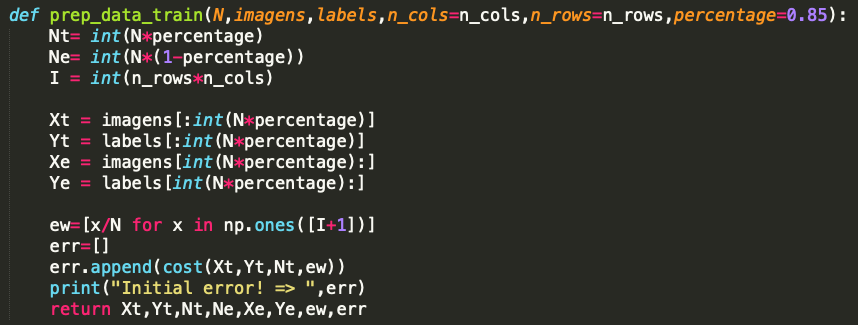
\includegraphics[width = \textwidth]{f_prep_data.png}
  
  \caption {Função de preparação dos datasets de treino e teste}
\end{figure}

\subsection{Classificador Logistico}


A implementação do classificador logistico foi dividida em 5 funções, nomeadamente: $run\_stocastic$, $predictor$, $sigmoid$, $cost$ e $update$ . Estas funções e respetivos funcionamentos serão apresentados em seguida pela ordem em que foram referidos.\newline



\subsubsection{Run Stocastic}\hfill\newline
	\hfill\newline

	A função run\_stocastic trata-se da função principal da implementação do classificador logistico e tal como o nome indica aplica o método estocástico ao mesmo. O método estocástico foi escolhido porque se trata do método que apresenta o menor custo em termos de performance face ás restantes tecnologias\cite{ref6,ref7}.\newline
	Esta função começa por definir que o erro almejado tem valor 0, indicando assim uma das condições de paragem do ciclo. Começa também por criar um contador $it$ para contabilizar as iterações realizadas inicializando este a 0.\newline
	A cada iteração é escolhido um elemento aleatório da nossa base de dados de treino e é calculado um novo vetor de pesos recorrendo á função $update$. Este novo vetor é posteriormente utilizado para calcular um erro através da função custo que indica a diferença entre os valores das labels calculados com recurso aos novos pesos e os valores reais das labels, sendo este erro armazenado para posterior visualização. A variável $it$ é então incrementada em 1 unidade e caso tenha atingido o número máximo de iterações que pretendemos sai do ciclo. 
	No final é devolvido o array de pesos juntamente com o array que contêm a progressão dos erros ao longo das iterações realizadas.

	\begin{figure}[H]

	  \centering
	  \captionsetup{justification=centering}

	  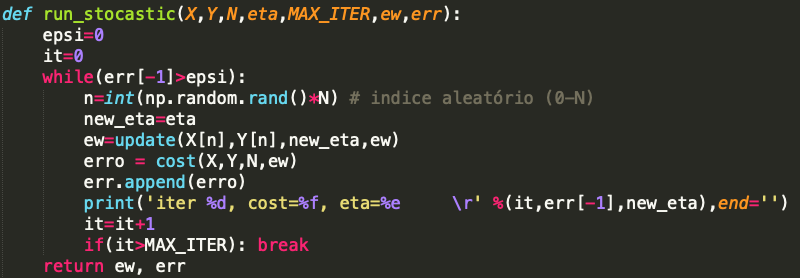
\includegraphics[width = \textwidth]{f_stocastic.png}
	  
	  \caption {Função Estocástica implementada}
	\end{figure}



\subsubsection{Predictor}\hfill\newline
	\hfill\newline

	A função predictor é responsável por calcular o valor em $\mathbb{R}$ a ser passado á função sigma. Este valor em $\mathbb{R}$ é calculado fazendo a soma do primeiro elemento do vetor de pesos pelo produto vetorial dos restantes elementos desse vetor com o array de pixeis representativo da imagem. No fim é devolvido o resultado de sigma.

	\begin{figure}[H]

	  \centering
	  \captionsetup{justification=centering}

	  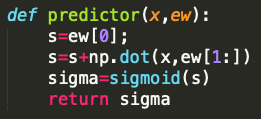
\includegraphics[width = 0.4\textwidth]{f_predictor.png}
	  
	  \caption {Função Predictor implementada}
	\end{figure}


\subsubsection{Sigmoid}\hfill\newline
	\hfill\newline
	Para a sua implementação recorreu-se á biblioteca python $numpy$ que possui uma função $numpy.exp()$ que recebe um expoente $s$ e calcula $e^s$, no entanto foi necessário ter atenção á capacidade de precisão do computador\footnote{A capacidade de precisão do computador refere-se ao número máximo de bits disponíveis para a representação de um número, exceder esta capacidade leva a erros de \textit{Overflow}.} e por esse motivo criaram-se limites de expoente de forma a que este não excedesse os números 30 e -30. \newline
	Nesta função o valor de s é arredondado mediante a necessidade, como referido no parágrafo anterior, e é usado como expoente de $\epsilon$ na função $\sigma$ devolvendo o resultado da mesma.

	\begin{figure}[H]

	  \centering
	  \captionsetup{justification=centering}

	  \includegraphics[width = 0.5\textwidth]{f_sigmoid.png}
	  
	  \caption {Função Sigmoid implementada}
	\end{figure}


\subsubsection{Cost}\hfill\newline
	\hfill\newline
	Esta função começa por criar um acumulador para os erros de predição das labels das imagens face ás labels reais chamado $En$ que é inicializado a 0 e pelos mesmos motivos de precisão computacional da função sigmoid establece um limite mínimo e máximo para o valor previsto.\newline
	Em seguida é iterado todo o dataset de treino imagem a imagem e sobre cada uma é calculada a probabilidade de esta imagem pertencer á label 1 e é utilizada a formula $Y_n*\log_\epsilon(\hat(y))+(1-Y_n)*\log_\epsilon{1-\hat(y)}$ para calcular o desvio da predição somando-o á variável $En$.\newline
	No fim é devolvida a média dos erros dividindo os erros acumulados pelos número de imagem iteradas.

	\begin{figure}[H]

	  \centering
	  \captionsetup{justification=centering}

	  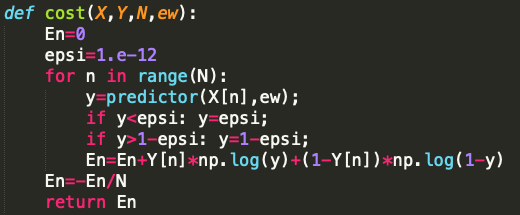
\includegraphics[width = 0.7\textwidth]{f_cost.png}
	  
	  \caption {Função Cost implementada}
	\end{figure}


\subsubsection{Update}\hfill\newline
	\hfill\newline
	A função update começa por obter uma predição sobre uma imagem e calcula a diferença entre o valor real da label da imagem e o valor previsto guardando-o na variável $s$. A variável $eta$ representa o learning rate a ser usado na atualização dos pesos.\newline
	 Posteriormente o primeiro elemento do array de pesos é atualizando somando-se ao produto de $s$ por $eta$ e os restantes elementos do array de pesos são atualizados individualmente somando-se ao produto de $s$ com $eta$ com o elemento da imagem x que se encontra na mesma posição do array - 1.\newline
	No final é devolvido um array com os pesos atualizados.

	\begin{figure}[H]

	  \centering
	  \captionsetup{justification=centering}

	  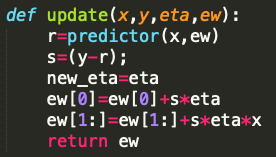
\includegraphics[width = 0.4\textwidth]{f_update.png}
	  
	  \caption {Função Update implementada}
	\end{figure}



\subsection{Poolings Clássicos}

 Nesta subsecção explicar-se-á a implementação das técnicas de pooling clássicas referidas na secção anterior. É de notar que a matriz a que cada pooling é aplicado foi transformada numa lista para uma mais facil implementação.


\subsubsection{Max Pooling}\hfill\newline
	\hfill\newline
	Este filtro aplica a função $max$ do python á lista recebida.

	\begin{figure}[H]

	  \centering
	  \captionsetup{justification=centering}

	  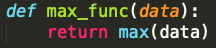
\includegraphics[width = 0.3\textwidth]{f_max.png}
	  
	  \caption {Função Max implementada}
	\end{figure}

\subsubsection{Min Pooling}\hfill\newline
	\hfill\newline

	Este filtro aplica a função $min$ do python á lista recebida.

	\begin{figure}[H]

	  \centering
	  \captionsetup{justification=centering}

	  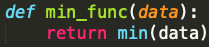
\includegraphics[width = 0.3\textwidth]{f_min.png}
	  
	  \caption {Função Min implementada}
	\end{figure}

\subsubsection{Average Pooling}\hfill\newline
	\hfill\newline

	Este filtor realiza uma divisão entre a soma dos elementos do vetor recebido e o tamanho do vetor recebido.


	\begin{figure}[H]

	  \centering
	  \captionsetup{justification=centering}

	  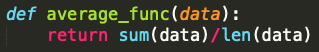
\includegraphics[width = 0.5\textwidth]{f_avg.png}
	  
	  \caption {Função Average implementada}
	\end{figure}

\subsubsection{Max Centered Pooling}\hfill\newline
	\hfill\newline

	Neste filtro utilizaram-se dois filtros préviamente definidos, subtraindo o resultado do filtro de average pooling ao resultado do filtro de max pooling. 


	\begin{figure}[H]

	  \centering
	  \captionsetup{justification=centering}

	  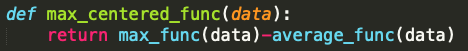
\includegraphics[width = 0.7\textwidth]{f_max_centered.png}
	  
	  \caption {Função Max centered implementada}
	\end{figure}



\subsection{Poolings Exóticos}\hfill\newline
\hfill\newline

Tal como já se referiu anteriormente foram criados alguns filtros de pooling exóticos baseados nas características do dataset de imagens. A sua implementação é decrita a seguir.

\subsubsection{ Diagonal and Vertical Average Pooling}\hfill\newline
  \hfill\newline

  A implemetação deste filtro passou por criar uma lista vazia denominada $lista$, uma variável $pos$\footnote{note-se que foi tirado partido do facto de a posição da diagonal ter as mesmas coordenadas em x e y, logo a variavel $pos$ representa tanto a linha da matriz em que estamos como a posição na linha em que o pixel se encontra.} a utilizar para iterar a posição do pixel a adicionar pertencente á diagonal da janela e uma variável $center$ que indica a posição do pixel de cada linha pertencente á vertical que se encontra no centro da janela.\newline
  Posteriormente é realizado um ciclo enquanto a posição do pixel diagonal for inferior a ambas as dimensões da janela. Em cada iteração, começa-se por adicionar á lista o pixel diagonal calculado como a posição do pixel diagonal na linha $pos$ somado com o número de pixeis por linha já percorrida. Em seguida acrescenta-se á lista o pixel pertencente á vertical calculado como a posição na linha correspondente á vertical dada pela variável $center$ somada ao número de pixeis percorridos nas linhas anteriores. Note-se que existe sempre um ponto em que a diagonal e a vertical se intersetam, o problema da dupla contabilização deste ponto foi resolvido com um if que impede que tal aconteça.\newline

   No final de cada iteração a linha, representada pela variável $pos$, é atualizada sendo incrementada em 1 unidade.\newline
  No fim da função retorna-se a média dos elementos da lista.

	\begin{figure}[H]

	  \centering
	  \captionsetup{justification=centering}

	  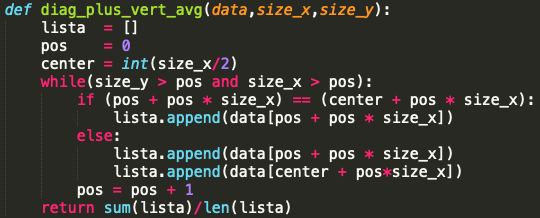
\includegraphics[width = 0.7\textwidth]{f_diag_plus_vert.png}
	  
	  \caption {Função que realiza a média sobre o filtro diagonal e vertical}
	\end{figure}


\subsubsection{Diagonal and vertical Max Centered Pooling}\hfill\newline
  \hfill\newline
  Esta função começa, tal como a anterior, por definir uma lista vazia, uma variável $pos$ e uma variável $center$ seguindo-se a coleta dos elementos da diagonal superior e da vertical da janela durante o ciclo que se segue. No final é devolvida a diferença entre o valor máximo da lista e a média dos valores da mesma.


    \begin{figure}[H]

	  \centering
	  \captionsetup{justification=centering}

	  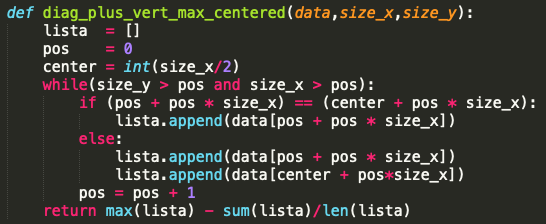
\includegraphics[width = 0.7\textwidth]{f_diag_plus_vert_max_centered.png}
	  
	  \caption {Função que realiza o "Max centered" sobre filtro diagonal e vertical}
    \end{figure}


\subsubsection{Diagonal and Vertical Max Pooling}\hfill\newline
  \hfill\newline
  	Nesta função são declaradas 3 listas, sendo que cada uma vai conter os elementos de uma das diagonais ou os elementos da reta vertical que se encontra no centro da janela. É também declarada uma variável $pos$ e uma variável $center$ á semelhança dos restantes filtros exóticos.\newline
  	Durante o ciclo os elementos da diagonal decrescente são colecionados no array $diag1$, os elementos da diagonal crescente no array $diag2$ sendo os elementos da vertical armazenados no array $vert$. \newline
  	Após o ciclo é encontrado o valor mínimo de cada um dos 3 arrays e desses é devolvido o maior.


	\begin{figure}[H]

	  \centering
	  \captionsetup{justification=centering}

	  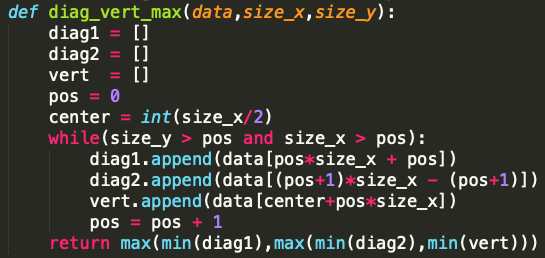
\includegraphics[width = 0.8\textwidth]{f_diag_vert_max.png}
	  
	  \caption {Função que obtem o maximo valor dos 3 valores mínimos encontrados nas diagonais e vertical do vetor}
	\end{figure}


\subsubsection{Diagonal and Vertical Min Average Pooling}\hfill\newline
  \hfill\newline
  Nesta função á semelhança da anterior declararam-se 3 listas, uma variavel $pos$ e uma variável $center$ que desempenham o mesmo papel que na função anterior. A coleta e armazenamento dos elementos das diagonais e da coluna central da janela também foram realizadas da mesma forma que na função anterior.\newline
  Após o ciclo foi calculada a média de cada lista e foi devolvida a menor média das três.

	\begin{figure}[H]

	  \centering
	  \captionsetup{justification=centering}

	  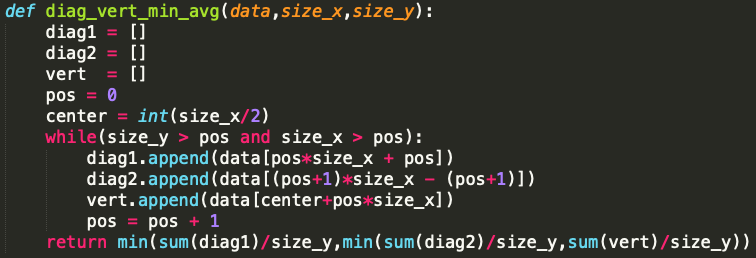
\includegraphics[width = \textwidth]{f_diag_vert_min_avg.png}
	  
	  \caption {Função que obtem o minimo valor das 3 médias calculadas sobre as diagonais e vertical do vetor}
	\end{figure}


Foi ainda definida uma função que permite simplificar a escolha do filtro a ser usado, ou seja, dada uma opção numérica, aplica o filtro associado ao vetor representativo da janela deslizante.

\begin{figure}[H]

  \centering
  \captionsetup{justification=centering}

  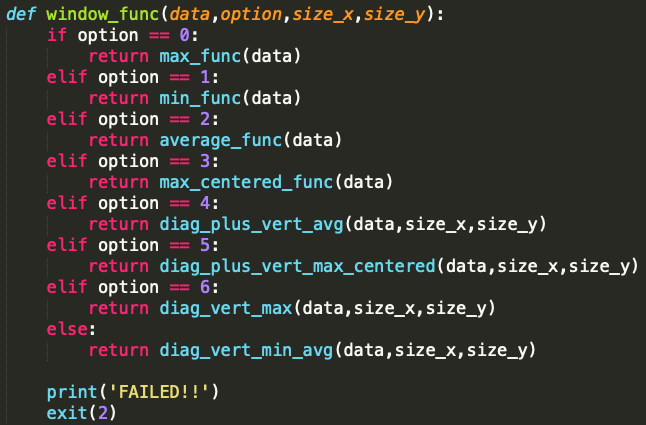
\includegraphics[width = 0.8\textwidth]{f_windows.png}
  
  \caption {Função responsável por fazer a correspondência opção-filtro}
\end{figure}


\subsubsection{Janela Deslizante}\hfill\newline
    \hfill\newline

	Foi implementada uma função responsável por aplicar a janela deslizante a cada imagem do dataset de forma genérica.\newline
	Esta função começa por definir as dimensões da imagem pós-filtro calculando quantas vezes tem de somar o $stride\_x$ á dimensão $x$ da janela deslizante para atingir o mesmo número de colunas que a imagem original e o mesmo processo é aplicado para calcular as dimensões em $y$ da imagem pós-filtro, fazendo uso da dimensão $y$ da janela, da variavel $stride\_y$ e da dimesão em $y$ da imagem pré-filtro\cite{ref8}.\newline
	Posteriormente os vetores representativos das imagens originais são iterados um a um e para cada são calculadas as posições abrangidas pela janela a cada iteração começando no ponto inicial (0,0) até a janela ter percorrido a totalidade da imagem. A cada uma das referidas iterações, nas quais se movimenta a janela, os pixeis abrangidos pela janela são armazenados num vetor ao qual se aplica um filtro para obter o valor de um pixel que passará a integrar a imagem pós-filtro.\newline
	O novo dataset constituido pelas imagens pós-filtro é então devolvido pela função.


	\begin{figure}[H]

	  \centering
	  \captionsetup{justification=centering}

	  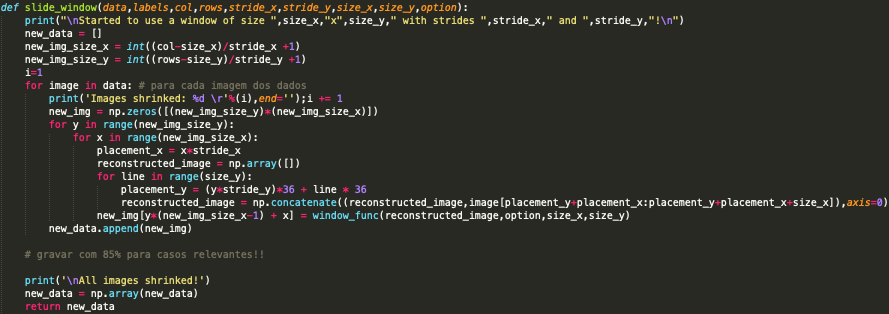
\includegraphics[width = \textwidth]{f_slidewindow.png}
	  
	  \caption {Função responsável por executar a janela deslizante}
	\end{figure}


\subsection{Avaliação de Resultados}

Para avaliar os modelos criados foi implementada uma função que calcula a matriz de confusão. Uma vez que no dataset utilizado classificar mal um 3 e classificar mal um 8 tem o mesmo peso a métrica Accuracy é a ideal para avaliar a qualidade das previsões do modelo, as métrica de Recall, Precisão e F-Score não são as melhores a aplicar uma vez que atribuem inportancias diferentes á classificação errónea de um 3 ou um 8.

\subsubsection{Matriz de Confusão}\hfill\newline
\hfill\newline

Esta função começa por criar a matriz 2x2 onde serão contabilizados os resultados da previsão das diversas imagens consoante se enquadrem nas definições dadas para o preenchimento de cada campo da matriz. Note-se que cada camp é inicializada a 0.\newline
As imagens da dataset são iteradas uma a uma e para cada é realizada um previsão. Posteriormente é contabilizado na tabela de confusão um dos quatro resultados:
\begin{itemize}
  \item Caso a previsão seja inferior a 0.5 e a label também a posição (0,0) da matriz é incrementada em um unidade.
  \item Caso a previsão seja superior a 0.5 e a label também a posição (1,1) da matriz é incrementada em um unidade.
  \item Caso a previsão seja inferior a 0.5 e a label seja superior a 0.5 a posição (0,1) da matriz é incrementada em um unidade.
  \item Caso a previsão seja superior a 0.5 e a label não a posição (1,0) da matriz é incrementada em um unidade.
\end{itemize}

\begin{figure}[H]

  \centering
  \captionsetup{justification=centering}

  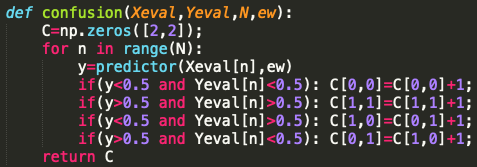
\includegraphics[width = 0.8\textwidth]{f_confusao.png}
  
  \caption {Função que calcula a matriz de confusão}
\end{figure}


\subsubsection{Accuracy}\hfill\newline
\hfill\newline

A implementação da accuracy passou por calcular usando a matriz de confusão quais as amostras corretamente classificadas e incorretamente classificadas pela ordem referida. e em seguida devolver o resultado da divisão do número de amostras bem classificadas pela totalidade das amostras classificadas (amostras bem classificadas + amostras mal classificadas).

\begin{figure}[H]

  \centering
  \captionsetup{justification=centering}

  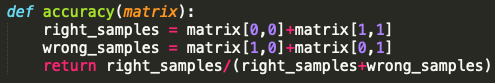
\includegraphics[width = 0.8\textwidth]{f_accuracy.png}
  
  \caption {Função que calcula a accuracy}
\end{figure}






























